\documentclass{beamer}
\mode<presentation>{\usetheme{DUR}}
\usepackage{amsmath}
\usepackage{cleveref}
\usepackage{wrapfig}
\usepackage[orientation=landscape,size=a2,scale=1.4,grid,debug]{beamerposter}

\newcommand{\defn}[1]{\textit{\color{ETH10}#1}}

\title{Assessing Insurance Risk}
\author[Ben Willis]{Ben Willis\\\normalsize{ Supervisor: Dr Matthias Troffaes}}
\institute{Durham University}
\date{\today}
\begin{document}
\begin{frame}
\begin{columns}
	\begin{column}{0.30\paperwidth}

		\begin{block}{Insurance Data Set}

			Classifiers have many applications in the finance industry ranging from financial trading to credit card fraud detection.
			We will study the problem of assessing the risk of insuring an automobile. \vspace{0.5em}

			\begin{center}
				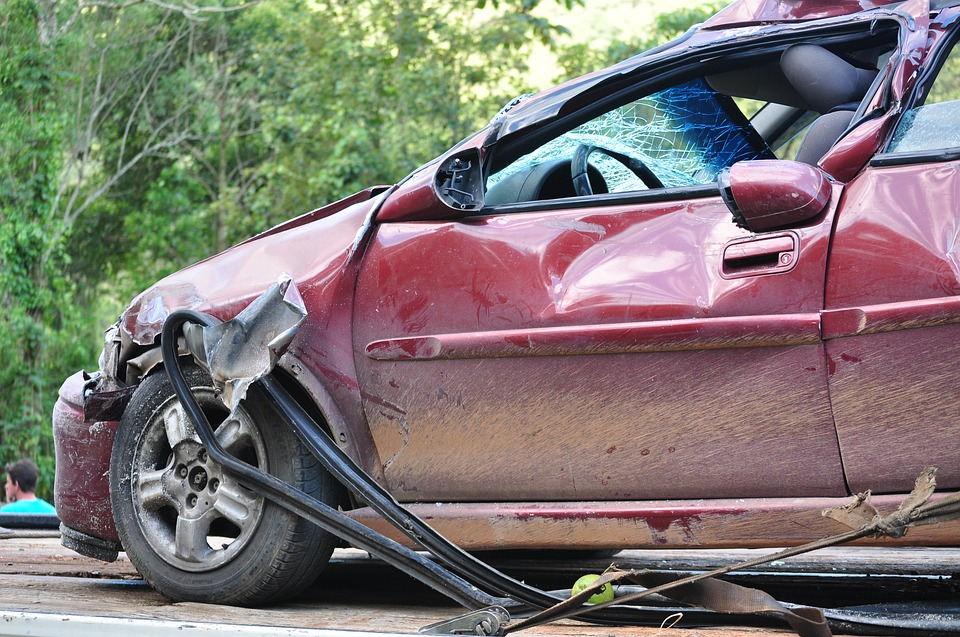
\includegraphics[width=.4\textwidth, keepaspectratio]{img/crash}
			\end{center}

			We will analyse a data set containing the technical attributes of 205 vehicles as well an expert's insurance risk rating.
			This rating is on an integer scale from -2 to 3 with 3 being most risky \cite{Automobile}.

			\begin{center}
				\begin{tabular}{l c c c c|r}
					Make       & Length & $\dots$ & Horsepower & Price & Risk \\
					\hline
					Volvo      & 188.8  & $\dots$ & 114        & 12940 & -2   \\
					Audi       & 192.7  & $\dots$ & 110        & 18920 & 2    \\
					Mitsubishi & 172.4  & $\dots$ & 116        & 9279  & 1    \\
					Audi       & 176.6  & $\dots$ & 115        & 17450 & ?
				\end{tabular}
			\end{center}

			We want to be able to accurately predict the risk of a vehicle given its technical information.
		\end{block}

		\begin{block}{Naive Bayes Classifier}
			The \defn{naive Bayes classifier} is a simple probabilistic approach to this classification problem that naively assumes each attribute is conditionally independent given the class.
			We are interested in $P(c \mid \mathbf{a})$, the probability of an automobile with attributes $\mathbf{a}$ having risk rating $c$.
			We use \defn{Bayes theorem} and the \defn{naivety assumption} to rewrite this probability:
			\begin{equation}
				P(c \mid \mathbf{a}) \propto P(c)P(\mathbf{a} \mid c) = P(c)\prod_{i=1}^{k}P(a_i \mid c)
			\end{equation}
			One way to assign a risk rating to a vehicle with attributes $\mathbf{a}$ is to choose the rating which maximises $P(c \mid \mathbf{a})$:
			\begin{equation} \label{map_estimate}
				\arg\max_{c \in \mathcal{C}} P(c \mid \mathf{a}) = \arg\max_{c \in \mathcal{C}} P(c)\prod_{i=1}^{k}P(a_i \mid c)
			\end{equation}
			This is known as the \defn{maximum a posteriori (MAP) estimate} and minimizes expected 0-1 loss.

			Alternatively, as our classes are numeric, we can choose the posterior expectation:
			\begin{equation}
				E(c \mid \mathbf{a}) = \sum_{c \in \mathcal{C}} c \cdot P(c \mid \mathf{a})
			\end{equation}
			This minimizes expected quadratic loss and is called the \defn{minimum mean square error (MMSE) estimate}.

		\end{block}

	\end{column}

	\begin{column}{0.38\paperwidth}

		\begin{block}{Likelihood Function}
			Now that we have our decision mechanism we need to estimate the required probabilities.
			We parametrise these probabilities:
			\begin{description}
				\item[\theta_c] Chance of a vehicle having risk rating $c$
				\item[\theta_{a_i \mid c}] Chance of a vehicle having attribute $a_i$ given that it has risk rating $c$
			\end{description}\vspace{0.5em}

			Given $N$ observations we denote the observed frequencies:
			\begin{description}
				\item[n(c)] Number of vehicles with risk rating $c$
				\item[n(a_i, c)] Number of vehicles with attribute $a_i$ and risk rating $c$
			\end{description}
			Note that $\sum_{c \in \mathcal{C}}n(c) = N$ and $\sum_{a_i \in \mathcal{A}_i}n(a_i, c) = n(c)$.\vspace{0.5em}

			The likelihood function for these theta chances given our observations is \cite{Zaffalon01}:
			\begin{equation} \label{likelihood}
				l(\mathbf{\theta} \mid \mathbf{n}) \propto \prod_{c \in \mathcal{C}} \left[ \theta_c^{n(c)} \prod_{i=1}^k \prod_{a_i \in \mathcal{A}_i} \theta_{a_i \mid c}^{n(a_i, c)} \right]
			\end{equation}
		\end{block}

		\begin{block}{Prior Distribution}
			We choose the following to be the prior distribution for our probabilities:
			\begin{equation} \label{prior}
				f(\mathbf{\theta} \mid \mathbf{t}, s) \propto \prod_{c \in \mathcal{C}} \left[ \theta_c^{st(c) - 1} \prod_{i=1}^k \prod_{a_i \in \mathcal{A}_i} \theta_{a_i \mid c}^{st(a_i, c) - 1} \right]
			\end{equation}
			where $s>0$ and $t(\cdot)$ are such that:
			\begin{equation}
				\sum_{c \in \mathcal{C}} t(c) = 1 \qquad \sum_{a_i \in \mathcal{A}_i} t(a_i, c) = t(c)  \ \forall \  i, c \qquad t(a_i, c) & > 0  \ \forall  \ i, a_i, c
			\end{equation}
			This distribution is the conjugate prior for our likelihood so the posterior distribution is in the same form as the prior.
			If the prior has hyperparameters $st(\cdot)$ the posterior will have hyperparameters $st(\cdot) + n(\cdot)$.\vspace{0.5em}

			Our prior beliefs about $P(c)$ and $P(a_i \mid c)$ are represented by $t(c)$ and $t(a_i , c)$.
			For now we want our prior to be indifferent towards each class so we set it to be uniform by choosing hyperparameters:
			\begin{equation}
				s = 1 \qquad t(c) = \frac{1}{|\mathcal{C}|} \qquad t(a_i, c) = \frac{1}{|\mathcal{A}_i||\mathcal{C}|}
			\end{equation} 
		\end{block}

		\begin{block}{Estimating Probabilities}
			One way to estimate the required probabilities is by choosing the theta values which maximise the likelihood.
			These are the \defn{maximum likelihood estimates} and are given by:
			\begin{equation}\label{mles}
				\hat{\theta}_c = \frac{n(c)}{N} \qquad
				\hat{\theta}_{a_i \mid c} = \frac{n(a_i, c)}{n(c)}
			\end{equation}\vspace{0.5em}

			Alternatively we multiply the likelihood by our prior and take the \defn{posterior expectation} \cite{Zaffalon01}:
			\begin{equation}
				E(\theta_c \mid \mathbf{n},s,\mathbf{t}) = \frac{n(c) + st(c)}{N + s} \qquad E(\theta_{a_i \mid c} \mid \mathbf{n},s,\mathbf{t}) = \frac{n(c) + st(a_i, c)}{N + st(c)}
			\end{equation}
		\end{block}

		
	\end{column}

	\begin{column}{0.25\paperwidth}

		\begin{block}{Application}
			We first discretize continuous variables and, as we have no mechanism for dealing with missing values, we discard any vehicles which are missing attributes.\vspace{0.5em}

			We will measure three metrics:
			\begin{description}
				\item[Accuracy] The percentage of correct risk rating assignments.
				\item[Random Assignments] The percentage of vehicles for which the classifier randomly assigns a class (when $P(c \mid \mathbf{a}) = 0$ for all $c$).
				\item[Mean Square Error] The average squared difference between the assigned class and true class; this measures closeness.
			\end{description}\vspace{0.5em}
		\end{block}

		\begin{block}{Results}
			Initially we use the MAP estimate for assigning a class and we compare the different estimates for the probabilities:
			\begin{center}
				\begin{tabular}{ l|c c }
					                      & Accuracy & Random Assignments\\
					\hline
					Maximum Likelihood    & 59.95\%  & 22.45\% \\
					Posterior Expectation & 68.17\%  & 0\%
				\end{tabular}
			\end{center}
			Using the prior leads to more accurate classifications and never assigns classes at random.

			Next we see how our method for assigning the risk rating affects the mean square error. We use the prior expectation for the probabilities to avoid random assignments
			\begin{center}
				\begin{tabular}{ l|c }
					              & Mean Square Error   \\
					\hline
					MAP Estimate  & 0.642 \\
					MMSE Estimate & 0.565
				\end{tabular}
			\end{center}
			Minimizing the expected quadratic loss reduces the mean square error as expected however this estimate may not be an integer.

			The next step is to investigate how sensitive our classifier is to changes in our prior distribution and consider whether our prior beliefs are really represented by indifference.
			We could also explore more decision mechanisms for assigning the class as well as ways to deal with missing values.
		\end{block}

		\begin{block}{\small References}
			{\footnotesize
			\bibliography{refs}{}}
			\bibliographystyle{abbrv}
		\end{block}

	\end{column}
\end{columns}
\end{frame}
\end{document}